\documentclass[aspectratio=169]{beamer}
% \setbeameroption{show notes on second screen}

\usepackage{lmodern}
\usepackage{array}
\usepackage{romannum}
\usepackage{amsmath}
\usepackage[overridenote, duration=10]{pdfpc}

\beamertemplatenavigationsymbolsempty
\setbeamertemplate{footline}[frame number]{}
\newcommand{\diff}{\operatorname{d}}

\newcommand{\overbar}[1]{\mkern 1.5mu\overline{\mkern-1.5mu#1\mkern-1.5mu}\mkern 1.5mu}
\title{PhD Application for CIMI \& EUR-MINT}
\author{Jianyu MA}
\date{\today}

\begin{document}

\frame{\titlepage}

\section{Academical curriculum vitae}

\begin{frame}
	\setbeamercovered{transparent}
	\frametitle{About Jianyu MA}
	\begin{table}
		\begin{tabular}{ >{\centering}m{10em} | c }
			Institution                                                & Internship Topic      \\
			\hline
			Wuhan University BS \newline UPS Toulouse \Romannum{3}  M1 & Stochastic calculus   \\
			\pause
			UPS Toulouse \Romannum{3}  M2                              & (Riemannian) geometry \\
		\end{tabular}
	\end{table}
	\setbeamercovered{invisible}
	\pause
	\begin{description}[A long description]
		\item[Research interest] Measure theory and Differential geometry \pause
			\note{
				You can tell this from my internship topics\\
			}
		\item[Work on] Convex analysis and Optimal transportation \pause
			\note{
				important in my internship\\
			}
		\item[Why IMT?] Common research interest with supervisor J.Bertrand

			Enjoyable environment, wonderful library, nice profs...
			\note{
				Reasons for IMT\\
			}
			\note{
				1. Important thing of PhD is to find somebody for a long time collaboration\\
				2. I include **scientific** environment in this sentence\\
			}
	\end{description}
\end{frame}

\section{Master Internship}
\begin{frame}
	\frametitle{Internship research topic}
	\begin{center}
		\huge Existence and uniqueness for \alert{barycenter} of probability measure
	\end{center}
\end{frame}

\subsection{Definition of barycenter}
\begin{frame}
	\frametitle{Heuristic definition}
	In mechanics, for a system of particles $m_\nu$ with positional vectors $\mathbf{r}_\nu$, the barycenter $c$ has positional vector
	\[
		\mathbf{r}_c := \sum_ { \nu } \frac{m_{\nu}}{M} \mathbf { r }_ { \nu } \equiv \arg \min_{\mathbf{r}} \sum_{\nu} \frac{m_\nu}{M} \Vert \mathbf{r}_{\nu} - \mathbf{r}\Vert^2
	\]
	where $ M := \sum _ { \nu } m _ { \nu } $, $\arg \min$: ``argument that achieves the minimum''.
	\note{
		Use **pointer**, save time\\
	}
	\note{
		1. An average of positional vectors r_v\\
		2. Coefficients proportional to mass \\
		3. Minimization problem of sum of square norms between r and r_v\\
	}
	\pause
	\begin{definition}
		For a probability measure $\lambda$ on a metric space $(E,d)$, barycenter $x \in E$ is
		\[
			x \in \arg\min_{z \in E} \int_{E} d^2(z,y) \diff \lambda(y)
		\]
	\end{definition}

	\note{
		Generalize from physics\\
	}

	\note{
		1. Norm square to distance square\\
		2. Sum of convex combination to probability measure integral
	}
\end{frame}

\subsection{Examples and my work}
\begin{frame}
	\frametitle{Ongoing work, part \Romannum{1}}
	\note{
		The **first part** of my work is to study examples\\
	}
	\begin{example}
		For $x,y \in E$, consider measure $\frac{1}{2}(\delta_x + \delta_y)$, if a barycenter $z$ exists,
		\[
			\text{barycenter} \equiv \text{midpoint}:\quad d(x, z) = d(z, y) = \frac{1}{2} d(x,y).
		\]
	\end{example}
	\pause
	\begin{block}{Remark}
		\begin{itemize}
			\item Points on equator are midpoints for north and south poles of a sphere. \pause

			      $\implies$ Barycenter: \alert{not unique} on the sphere \pause

			      \hspace{3.6em} Reason: the sphere has positive curvature  \pause


			\item In a complete space, midpoint exists $\iff$ shortest path exists.\pause

			      Example: no shortest path between north and south poles of

			      infinite dimensional ellipsoid with axes of decreasing length \pause

			      $\implies$ Barycenter: \alert{not always exists}
		\end{itemize}
		\note{
			Example of sphere\\
		}
		\note{
			1. Go back to this reason later\\
			2. Too much curvature: shortest path is not unique\\
			3. Cut locus: another geometric connection\\
		}
		\note{
			Finite ellipsoid, at least 2 barycenters: symmetry\\
		}
		\note{
			1. Infinite ellipsoid is not compact, like the unit sphere in Hilbert space\\
			2. Shift coordinates one step right and decrease them, we can always get shorter path than given one\\
		}
	\end{block}
\end{frame}

\begin{frame}
	\frametitle{Metricized space of measures on $\mathbb{R}^2$ }
	Images represent uniform probability measures on them.\\
	We regard images as points in our metric space.
	\note{
		Be **funny**\\
	}
	\begin{columns}
		\column<2->{0.5\textwidth}
		\begin{description}[explanation]
			\item[Space] Probability measures on $\mathbb{R}^2$
			\item[Metric] Wasserstein metric
			\item[Measure] $\frac{1}{2}(\delta_{\text{img1}} + \delta_{\text{img2}})$
			\item[Barycenter] Middle image of two images
		\end{description}
		\column{0.5\textwidth}
		\centering
		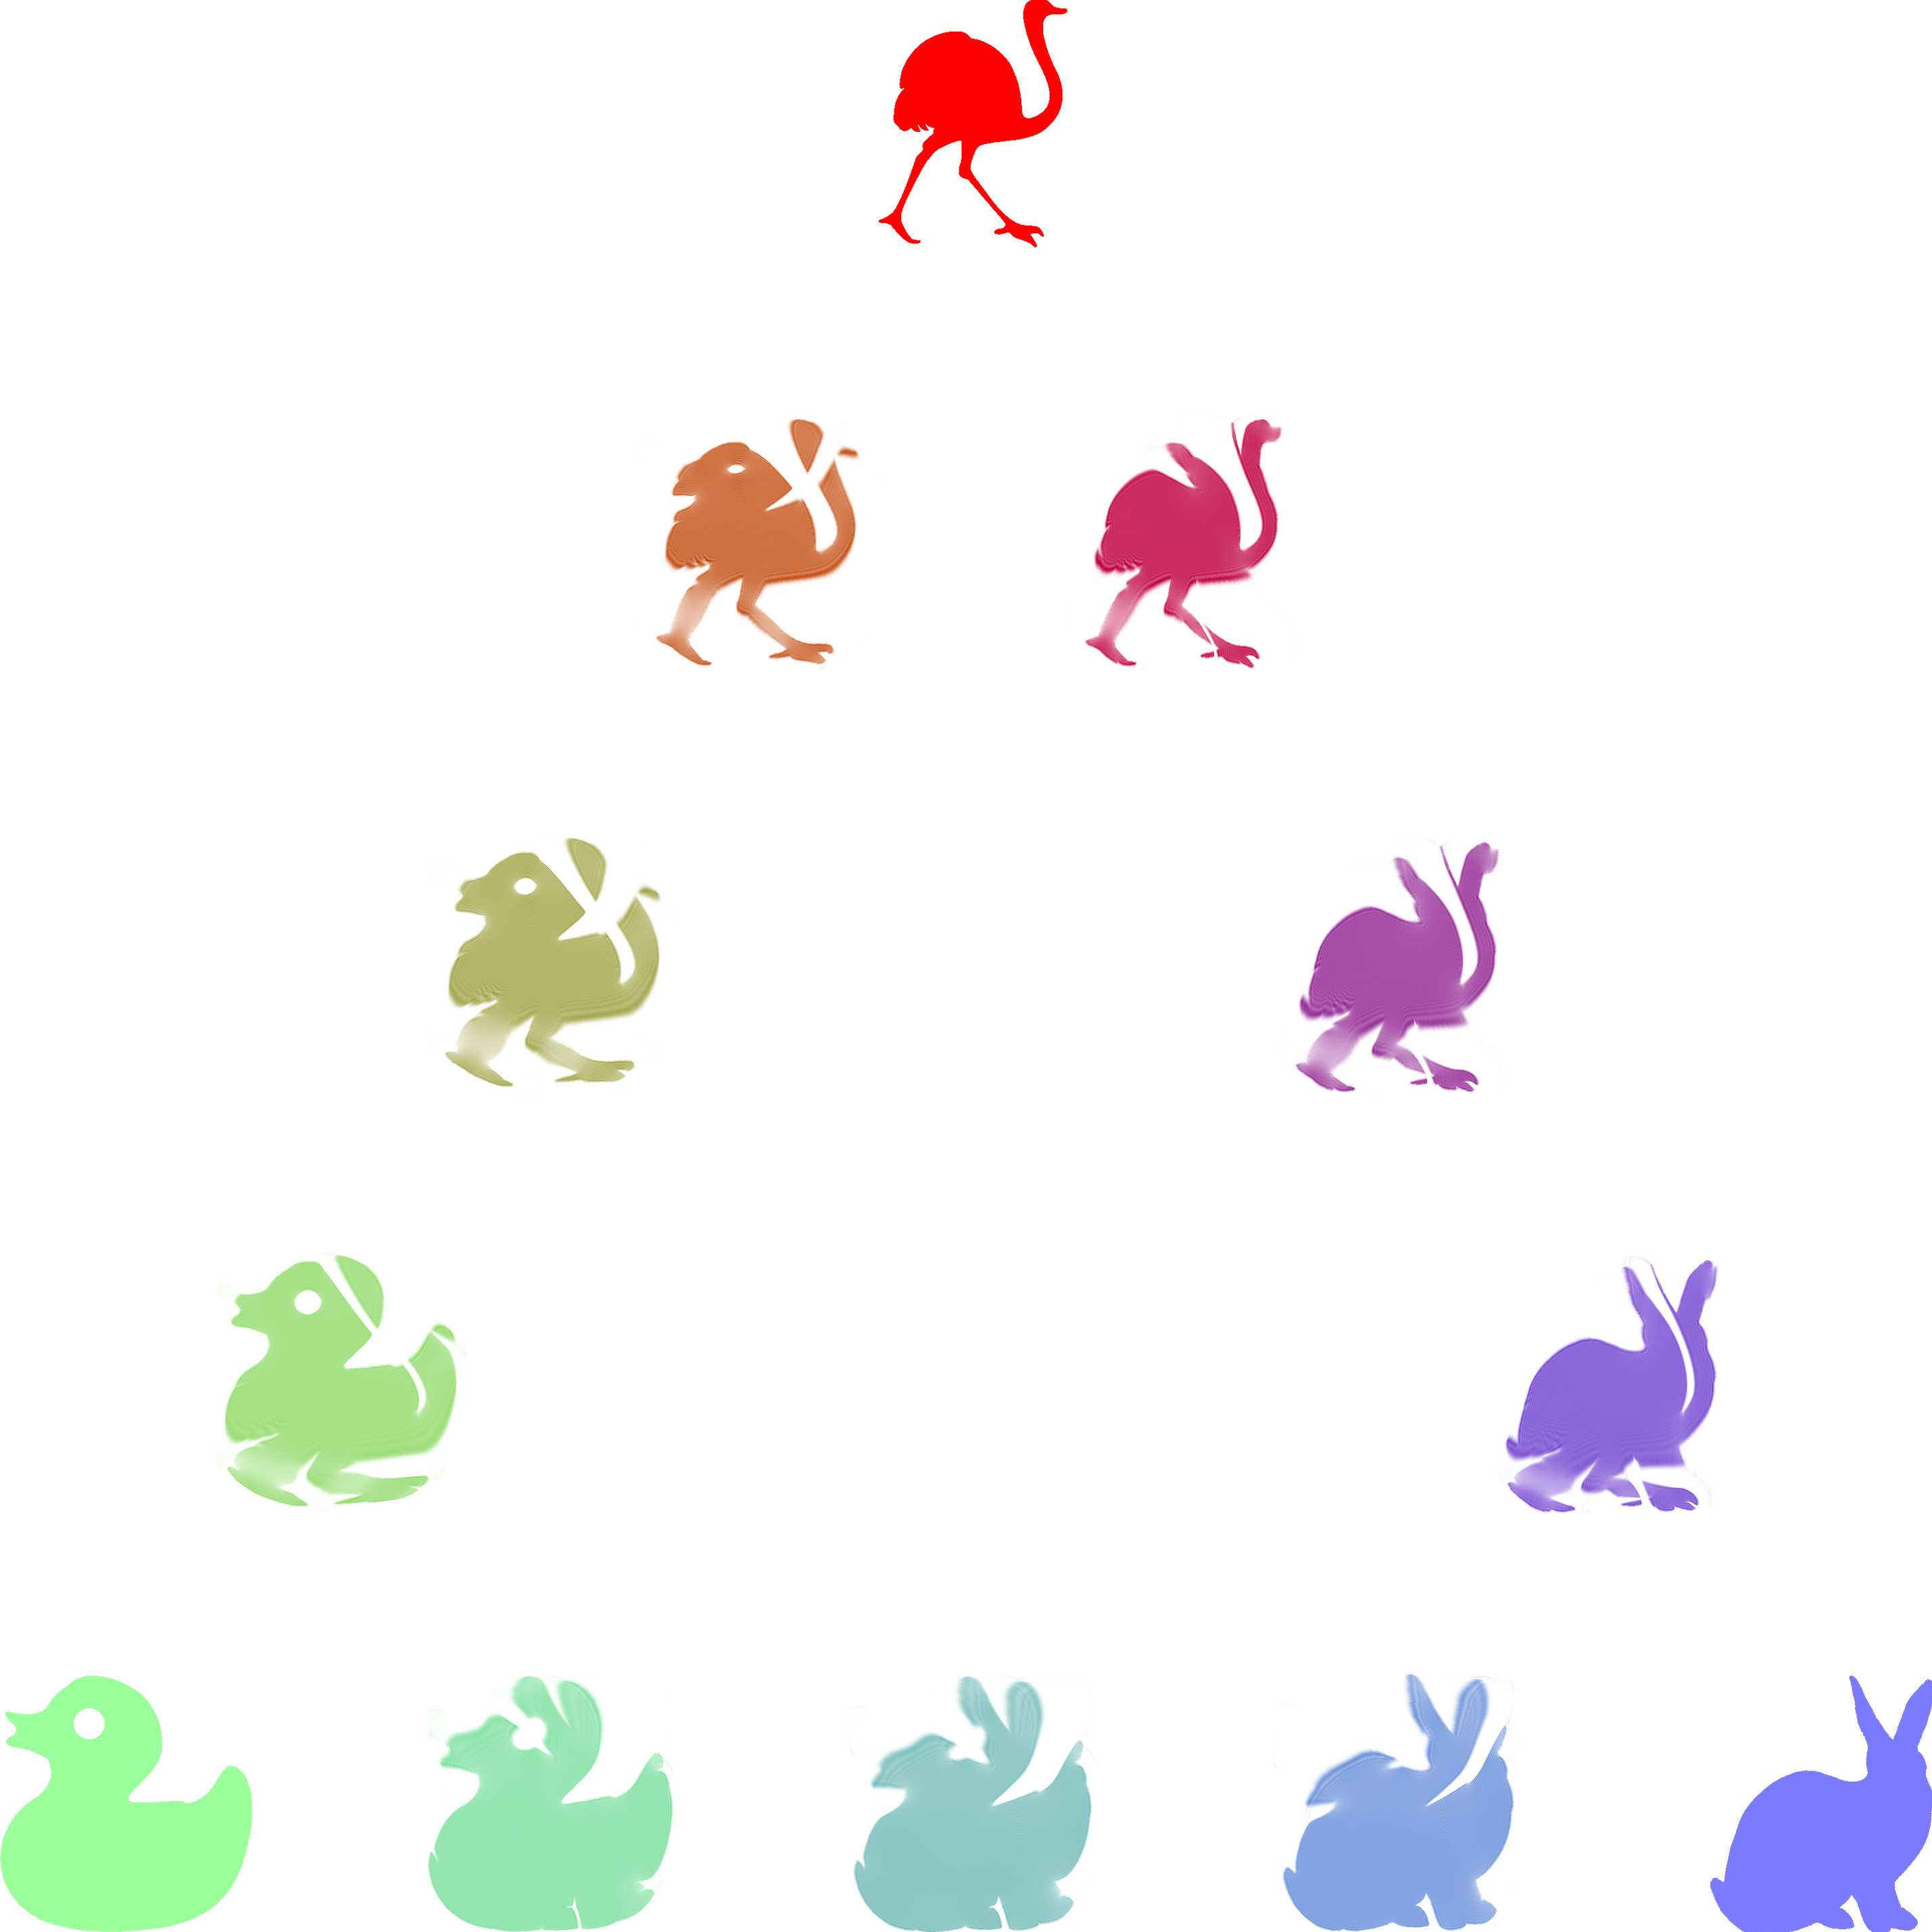
\includegraphics[height=6cm]{barycenter.png}
	\end{columns}
	\note{
		1. We place barycenter of two images in the middle\\
		2. It is a pun to say barycenter is midpoint\\
		3. Could have application in image process\\
	}
\end{frame}

\subsection{Internship overview}
\begin{frame}
	\setbeamercovered{invisible}
	\frametitle{Ongoing work, part \Romannum{2}}
	\begin{block}{Motivations from Statistical Inference}
		\note{
			Research is pure math, geometry and measure theory. **Application oriented**\\
		}
		\centering barycenter (of discrete measures) $\equiv$ Fréchet mean

		\pause
		\raggedright
		\begin{itemize}
			\item Empirical measures are discrete\pause
			\item Datasets without Euclidean structure
		\end{itemize}
		\note{
			1. Not new to statisticians, but my knowledge is limited\\
			2. Let's turn to some theoretical results\\
			3. Recently,	I have studied these results in detail\\
		}
	\end{block}
	\setbeamercovered{transparent}
	\pause
	\begin{block}{Results in the field}
		\pause
		\begin{tabular}{
			@{}
			>{\raggedleft}m{15em}
			c
			m{15em}
			@{}}
			Bounded sets are compact      & $\Rightarrow$ & Existence of barycenter\pause   \\
			Non-positive curvature        & $\Rightarrow$ & Uniqueness of barycenter\pause  \\
			Optimal transportation theory & inspires      & Barycenter on Wasserstein space \\
		\end{tabular}
	\end{block}
	\note{
		Minimization sequence are bounded\\
	}
	\note{
		Two ways to show uniqueness\\
	}
	\note{
		1. Triangle comparison inequality, take integral\\
		2. Square distance function is strongly convex\\
	}
	\note{
		Wasserstein space\\
	}
	\note{
		1. Example of images, as we talked just now\\
		2. Multi-marginal mass transport problem, barycenter on Wasserstein space\\
	}
	\setbeamercovered{invisible}
	\pause
	\begin{block}{Current progress: Convex analysis and Optimal transportation}
		\begin{itemize}
			\item Investigate the case of $\mathbb{R}^n$
			      \pause
			\item Generalize to Riemannian manifolds
		\end{itemize}
	\end{block}
			      \note{
				      Difficulties\\
			      }
			      \note{
				      1. Not my master courses\\
				      2. Study carefully to get inspiration\\
				      3. No linear structure, verify classic results in detail\\
			      }
\end{frame}

\section{PhD proposal}
\begin{frame}
	\frametitle{PhD research topic}
	\begin{center}
		\huge	Barycenter and Central Limit Theorem \normalsize (abbr. as CLT)
	\end{center}
\end{frame}

\subsection{Recall classic CLT}
\begin{frame}
	\frametitle{Recall classic CLT}
	\begin{block}{Central Limit Theorem}
		Draw $n$ independent random samples $X_1, X_2, \ldots, X_n$ from a population with overall mean $\mu$ and finite variance $\sigma^2$, denote by
		\[
			\overbar {X}_{n}:= \frac{X_1 + X_2 + \cdots + X_n}{n}
		\]
		the sample mean, we have
		\[
			\sqrt{n}\frac{\overbar {X}_{n}-\mu }{\sigma} \xrightarrow {\text{law}} N\left(0,1\right),
		\]
		where $N(0,1)$ is the standard normal distribution.
	\end{block}
	\note{
		1. X_i as samples, they have the same distribution\\
		2. Classic proof uses Fourier transform, not available on manifolds\\
		3. Alternative proof uses optimal transportation, possible to generalize\\
	}
\end{frame}
\subsection{Introduction to PhD proposal}
\begin{frame}
	\frametitle{CLT in terms of barycenter}
	\begin{center}
		\large Barycenter = Mean of measure on a metric space
	\end{center}
	\setbeamercovered{transparent}
	\pause
	\begin{block}{Crucial properties of barycenter to get CLT}
		\begin{description}[Long description]
			\item[Uniqueness] Converges to a unique mean
				\pause
			\item[Consistency] Convergence of measures $\implies$ Convergence of their barycenters
				\pause
		\end{description}
	\end{block}

	\begin{block}{Some metric spaces to investigate}
		\begin{enumerate}
			\item Riemannian manifolds
			      \pause
			\item Wasserstein space: measures on a metric space with finite second moments
		\end{enumerate}
		\note{
			Think barycenter as mean, we wonder if CLT holds in a more general setting\\
		}
		\note{
			In CLT, it is necessary of sample mean to converge point-wisely to a unique overall population mean\\
		}
		\note{
			1. Consistency holds on Wasserstein space\\
			2. CLT here is the study of converging behavior of barycenters\\
		}
		\note{
			Again we are interested in these two kinds of space\\
		}
		\note{
			1. Existence and uniqueness of barycenter on these spaces for internship topic\\
			2. CLT on these spaces for my PhD projects
		}
	\end{block}
\end{frame}
\end{document}
